
\begin{figure}[t]
\centering
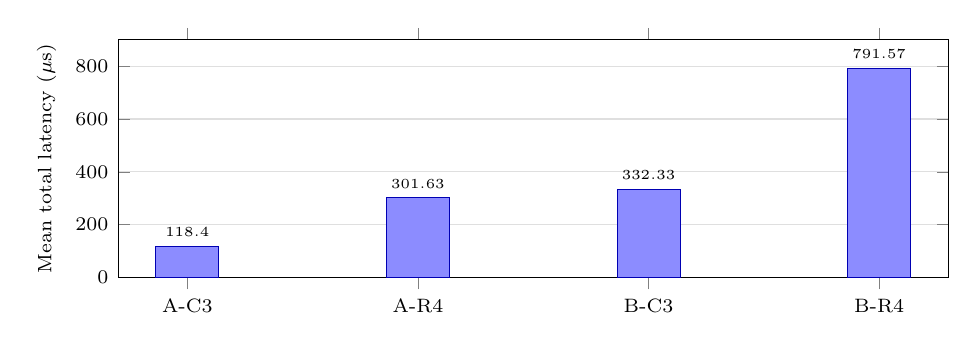
\begin{tikzpicture}
\begin{axis}[
  width=\columnwidth,height=46mm,ybar,bar width=8mm,
  symbolic x coords={A-C3,A-R4,B-C3,B-R4},xtick=data,
  ymin=0,ymax=900,ylabel={Mean total latency ($\mu$s)},
  nodes near coords,nodes near coords style={font=\tiny},
  tick label style={font=\scriptsize},label style={font=\scriptsize},
  ymajorgrids=true,major grid style={gray!25}
]
\addplot[fill=blue!45,draw=blue!70!black] coordinates {
 (A-C3,118.40) (A-R4,301.63)
 (B-C3,332.33) (B-R4,791.57) };
\end{axis}
\end{tikzpicture}
\caption{Measured fixed-point preprocessing-plus-inference latency over all 56,200 records. C3 denotes ESP32-C3 and R4 denotes Arduino UNO R4 WiFi.}
\label{fig:hil-latency}
\end{figure}
